\documentclass[a4paper, 10pt]{report}
\usepackage[italian]{babel}
\usepackage[T1]{fontenc}
\usepackage[utf8]{inputenc}
\usepackage{charter}
\usepackage{amsmath}
\usepackage{amsthm}
\usepackage{amsfonts}
\usepackage{graphicx}
\usepackage{wrapfig}
\usepackage{tcolorbox}
\usepackage{fancyhdr}
\usepackage{listings}
\usepackage{longtable}

\usepackage{geometry}
\geometry{a4paper, left=2cm,right=2cm,top=2cm,bottom=2cm}

\pagestyle{fancy}
\lhead{}
\chead{}
\rhead{\bfseries 30 ottobre 2019 }
\lhead{\bfseries Segnali e immagini}

\begin{document}
\section*{\underline{Analisi di Fourier}}
L'analisi di Fourier permette di passare da segnali temporali o spaziali a frequenziale e viceversa.

\subsection*{Serie di Fourier}
\paragraph*{Funzione di sintesi} Una funzione $f: R \rightarrow R$ periodica di periodo $T$, con variabile continua $t$, può essere espressa come:
\begin{align*}
f(t) = \sum_{n=-\infty}^{+\infty} c_ne^{j\frac{2 \pi n}{T} t} \hspace{1.5cm}\text{(sintesi)}
\end{align*}

\noindent con $n \in Z$. Praticamente la funzione di analisi sintetizza ol segnale come somma di molteplici oggetti. I coefficienti $c_n$ rappresentano i pesi, mentre le esponenziali $e^{j\frac{2 \pi n}{T} t}$ rappresentano le fratures/caratteristiche del signali (dipendono da $n$).

\paragraph*{Funzione di analisi} I coefficienti $c_n$ sono calcolati come segue:
\begin{align*}
c_n = \frac{1}{T} \int_{-\frac{T}{2}}^{+\frac{T}{2}} f(t)e^{-j\frac{2 \pi n}{T} t} \, dt \hspace{1.5cm}\text{(analisi)}
\end{align*}
\noindent per $n \in Z$. 

\paragraph*{Rappresentazione dei coefficienti} I coefficienti possono essere rappresentati nelle forma rettangolare ($c_n = Re + jIm$) oppure nella forma polare ($c_n = |c_n|e^{j\theta_n}$).
\begin{center}
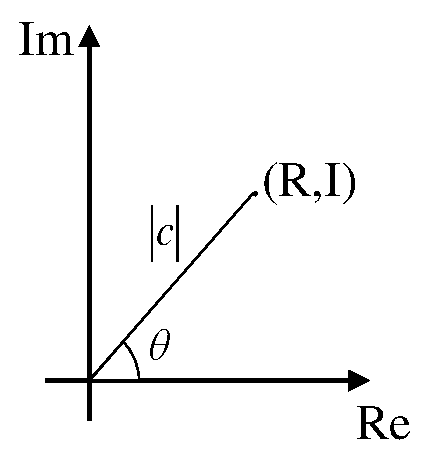
\includegraphics[scale=0.65]{1.pdf}
\end{center}

\paragraph*{Spiegazione della funzione di sintesi} L'esponenziale $e^{j\frac{2 \pi n}{T} t}$ viene interpretata come un fasore, dove $\frac{2 \pi n}{T} t$ rappresenta la sua velocità angolare\footnote{Più grande è $n$ (che dipende dal coefficiente $c_n$), più giri vengono effettuati nell'unità di tempo, e quindi più grande è la velocità angolare.}. 

\noindent Quindi ogni termine della sommatoria, ottenuto dalla moltiplicazione di un numero complesso e un fasore, sarà un altro fasore:
\begin{align*}
c_ne^{j\frac{2 \pi n}{T} t} = |c_n|e^{j\theta_n}e^{j\frac{2 \pi n}{T} t} = |c_n|e^{j\frac{2 \pi n}{T} t + \theta_n}
\end{align*}

\noindent In questo modo, praticamente, estendo il fasore iniziale $e^{j\frac{2 \pi n}{T} t}$ ad una lunghezza $|c_n|$, facendolo partire con un angolo $\theta_n$ (detto angolo di fase). 
\begin{center}
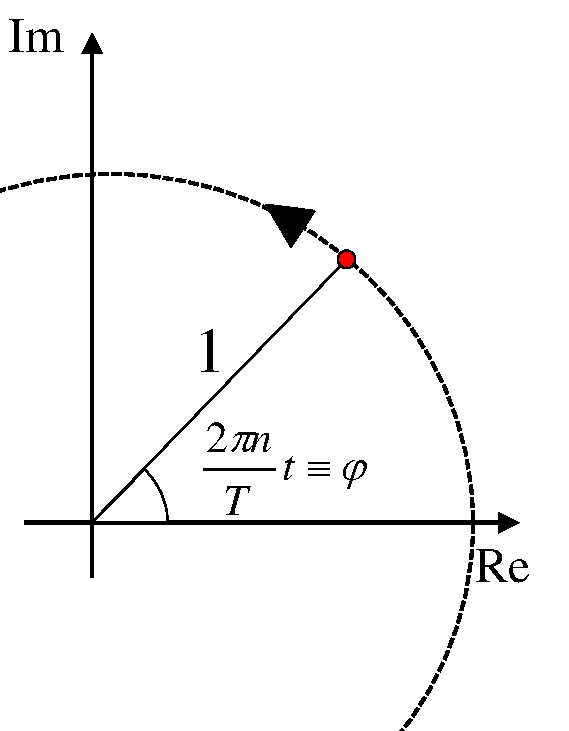
\includegraphics[scale=0.6]{2.pdf}

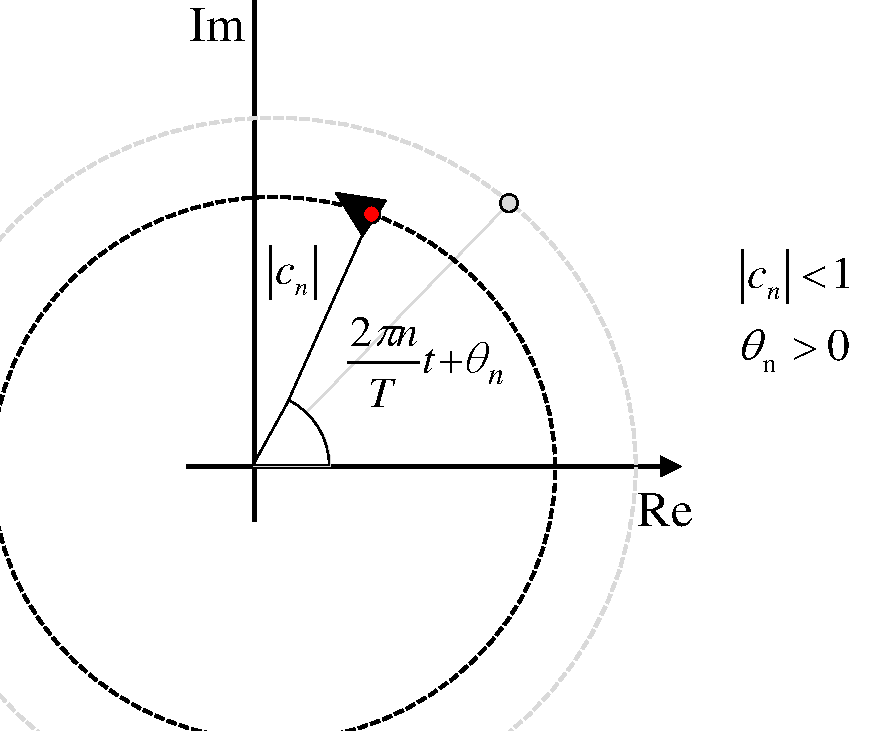
\includegraphics[scale=0.6]{3.pdf}
\end{center}
\vspace{1cm}
\begin{tcolorbox}[title=\textbf{Caso coefficiente reale}]
\begin{center}
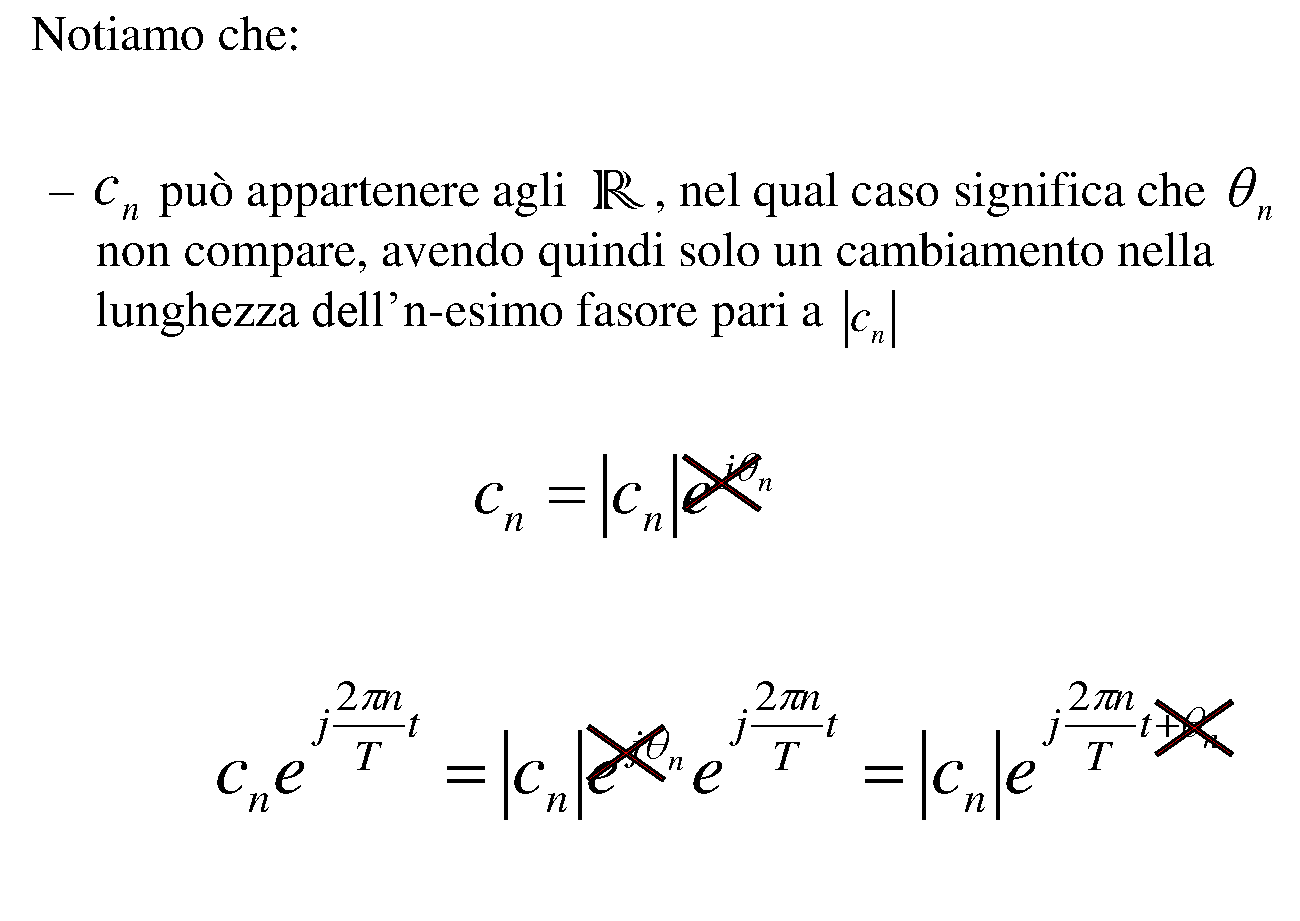
\includegraphics[scale=0.50]{reali.pdf}
\end{center}
\end{tcolorbox}

\paragraph*{Proprietà della serie di Fourier} Lo spettro di ampiezza e di fase sono funzioni nel dominio delle frequenze che formano lo spettro di Fourier. Nel caso di segnali periodici, lo spettro di Fourier gode delle seguenti proprietà:
\begin{itemize}
\item[-] Lo spettro di ampiezza è simmetrico rispetto all'asse y;
\item[-] Lo spettro di fase è antisimmetrico rispetto all'asse y;
\item[-] Se i coefficienti $c_n$ sono reale, allora lo spettro di fase non esiste;
\item[-] Entrambi gli spettri sono funzioni a pettine, definite su frequenze $\frac{2 \pi  n}{T}$, con $n \in Z$ (ovvero frequenze multiple rispetto a quella fondamentale $\frac{2 \pi}{T}$).
\end{itemize}









\end{document}